\section[Git Branching]{Git Branching}
\subsection[]{Overview}
\begin{frame}
\frametitle{Git Branching - Overview}
\begin{itemize}
	\item A branch represents an independent line of development.
	\item Lightweight implementation of branching – Git stores a branch as \textbf{a reference to a commit}.
	\item Keeps history as a tree, where \textbf{each commit is a node} in the tree, and has one or more parents.
	\item History is \textbf{extrapolated through the commit relationships}.
	\item It’s a good practice to \textbf{spawn a new branch to encapsulate your changes} no matter how big the changes are.
\end{itemize}
\end{frame}



\subsection[]{Local Branches}
\begin{frame}
\frametitle{Git Branching - Local Branches}
\begin{itemize}
	\item \textbf{Non-tracking local branches}
		\begin{itemize}
		\item Exist on user’s machine.
		\item Not associated with any other branch.
		\item User needs to specify which upstream branch when running push or pull commands.
		\end{itemize}
	\item \textbf{Tracking local branches}
		\begin{itemize}
		\item Exist on user’s machine.
		\item Tracking branch is a branch that has a direct relationship to another branch.
		\item Local tracking branches in most cases track a remote tracking branch.
		\item Allow user to run git pull and git push without specifying which upstream branch to use.
		\end{itemize}
\end{itemize}
\end{frame}

\subsection[]{Local Branches - remote-tracking branches}
\begin{frame}
\frametitle{Git Branching - remote-tracking branches}
\begin{itemize}
	\item \textbf{Remote}
		\begin{itemize}
		\item Remote connection (bookmark) into other repository.
		\end{itemize}
	\item \textbf{Remote branch}
		\begin{itemize}
		\item Branch on a remote location.
		\end{itemize}
	\item \textbf{Remote-tracking branch}
		\begin{itemize}
		\item Local cache for what the remote repositories contain.
		\item (remote)/(branch)
			\begin{itemize}
			\item origin/master
			\item origin/test-branch
			\end{itemize}
		\end{itemize}
	\item \textbf{Note:}
		\begin{itemize}
		\item “origin” and “master” are not special.
		\end{itemize}
\end{itemize}
\end{frame}

\subsection[]{Git Branching - merge}
\begin{frame}
\frametitle{Git Branching - merge}
\begin{itemize}
	\item Way of putting a forked \textbf{history back together} again.
	\item\textbf{Non-destructive} operation.
	\item All the operations always \textbf{merge into the current} branch.
	\item Git has \textbf{several distinct algorithms} to accomplish the merge.
\end{itemize}
Note:
\begin{itemize}
	\item git pull command effectively runs git fetch and git merge.
\end{itemize}
\end{frame}

\begin{frame}
\frametitle{Git Branching - merge}
\begin{itemize}
	\item \textbf{3-Way Merge}
		\begin{itemize}
		\item Creates \textbf{merge commit} that ties together the histories of both branches.
		\item Merge commit as a \textbf{symbolic joining} of the two branches.
		\item Original \textbf{context is maintained}.
		\end{itemize}
	\item \textbf{Fast-Forward Merge}
		\begin{itemize}
		\item Requires \textbf{linear path} from the current branch tip to the target branch.
		\item Usually \textbf{facilitated through rebasing} – suitable for small tasks and fixes.
		\item Context of the affected commits as part of an earlier feature branch is lost.
		\end{itemize}
\end{itemize}
\end{frame}

\subsection[]{Local Branches - 3-way merge}
\begin{frame}
\frametitle{Git Branching - 3-way merge}
\begin{tikzpicture}
  \node (img1) {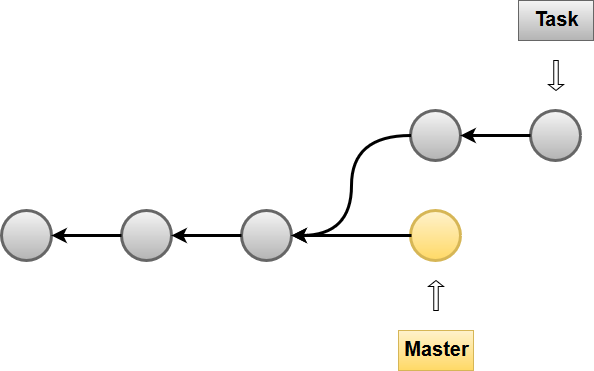
\includegraphics[width=6.4cm, height=4cm]{3waymerge-1.png}};
%  \pause
  \begin{scope}[on background layer]
  	\node (img2) at (img1.south east) [yshift=-1cm] {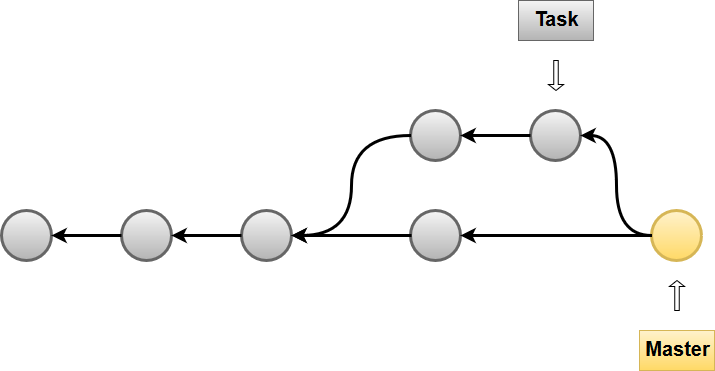
\includegraphics[width=7.7cm, height=4cm]{3waymerge-2.png}};
  \end{scope}
\end{tikzpicture}


\end{frame}

